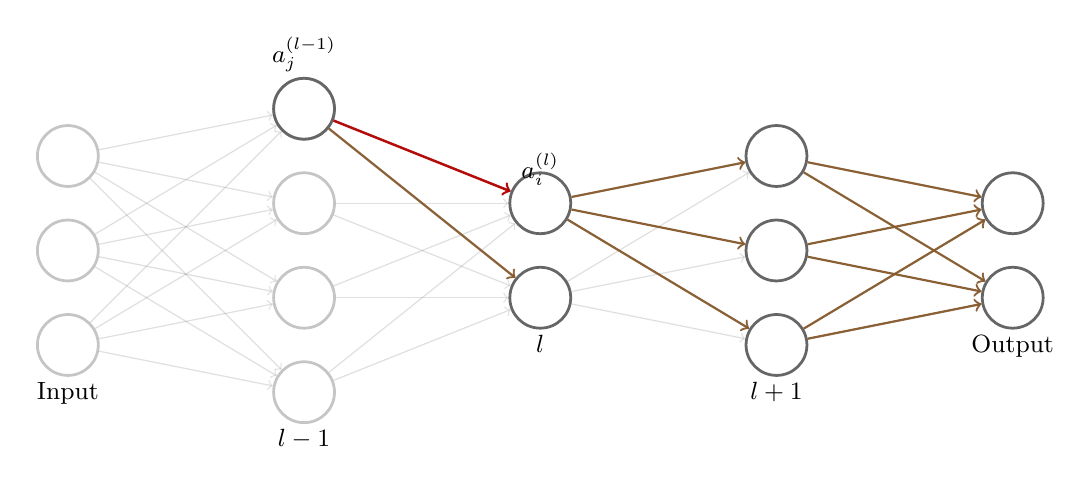
\begin{tikzpicture}[
  neuron/.style={circle, draw=black!60, line width=1.0pt, minimum size=22pt, inner sep=0pt},
  faded_neuron/.style={neuron, opacity=0.38},
  focus_neuron/.style={neuron, opacity=1.0},
  conn_faded/.style={->, draw=black!55, line width=0.45pt, opacity=0.22},
  conn_active/.style={->, draw=brown!70!black, line width=0.8pt, opacity=0.95},
  conn_weight/.style={->, draw=red!70!black, line width=0.9pt, opacity=0.95}
]

% Input layer (faded)
\foreach \i/\y in {1/1.2,2/0,3/-1.2} {
  \node[faded_neuron] (i\i) at (0, \y) {};
}

% Hidden layer 1 (top node in focus, rest faded)
\foreach \j/\y in {1/1.8,2/0.6,3/-0.6,4/-1.8} {
  \node[faded_neuron] (h1\j) at (3.0, \y) {};
}
\node[focus_neuron] (h11f) at (3.0, 1.8) {};

% Hidden layer 2 (both nodes in focus)
\foreach \j/\y in {1/0.6,2/-0.6} {
  \node[focus_neuron] (h2\j) at (6.0, \y) {};
}

% Hidden layer 3 (all in focus)
\foreach \j/\y in {1/1.2,2/0,3/-1.2} {
  \node[focus_neuron] (h3\j) at (9.0, \y) {};
}

% Output layer (in focus)
\foreach \k/\y in {1/0.6,2/-0.6} {
  \node[focus_neuron] (o\k) at (12.0, \y) {};
}

% --- Faded dense connections ---
\foreach \i in {1,...,3} {
  \foreach \j in {1,...,4} {
    \draw[conn_faded] (i\i) -- (h1\j);
  }
}
\foreach \i in {1,...,4} {
  \foreach \j in {1,...,2} {
    \draw[conn_faded] (h1\i) -- (h2\j);
  }
}
\foreach \i in {1,...,2} {
  \foreach \j in {1,...,3} {
    \draw[conn_faded] (h2\i) -- (h3\j);
  }
}
\foreach \i in {1,...,3} {
  \foreach \k in {1,2} {
    \draw[conn_faded] (h3\i) -- (o\k);
  }
}

% --- Highlighted path ---
% Red weight: h11f -> h21 and h11f -> h22
\draw[conn_weight] (h11f) -- (h21);
\draw[conn_active] (h11f) -- (h22);

% Brown active: from h21 -> all of HL3
\foreach \j in {1,...,3} {
\draw[conn_active] (h21) -- (h3\j);
}

% Brown active: all of HL3 -> all outputs
\foreach \i in {1,...,3} {
  \foreach \k in {1,2} {
    \draw[conn_active] (h3\i) -- (o\k);
  }
}

% --- Labels ---
\node[above=4pt]  at (3.0,  2)  {\small $a_j^{(l-1)}$};
\node[below=4pt]  at (6.0, 1.5)  {\small $a_i^{(l)}$};
\node[below=10pt] at (0,   -1.2)  {\small Input};
\node[below=10pt] at (3.0, -1.8)  {\small $l-1$};
\node[below=10pt] at (6.0, -0.6)  {\small $l$};
\node[below=10pt] at (9.0, -1.2)  {\small $l+1$};
\node[below=10pt] at (12.0,-0.6)  {\small Output};

\end{tikzpicture}